\chapter{Improving the FDTD Code \label{chap:fdtdImproved}} 

%\setcounter{page}{1}

\renewcommand{\thefootnote}{\fnsymbol{footnote}}
\footnotetext{Lecture notes by John Schneider.  {\tt
fdtd-improved-code.tex}}

\section{Introduction}

The C code presented in the previous chapter adequately served its
purpose---it implemented the desired FDTD functionality in a
relatively straightforward way.  However, as the algorithms get more
involved, for instance, when implementing simulations of two- or
three-dimensional problems, the readability, portability, and
maintainability will be improved if our implementation is slightly
more sophisticated.  In this chapter we will implement the algorithms
of the previous chapter in a way which may seem, at first, to be
overly complicated.  However, as the complexity of the algorithms
increases in coming chapters, we will see that the effort required to
understand this more sophisticated approach will have been worth it.

%%%%%%%%%%%%%%%%%%%%%%%%%%%%%%%%%%%%%%%%%%%%%%%%%%%%%%%%%%%%%%%%%%%%%%%%%%%
\section{Arrays and Dynamic Memory
  Allocation \label{sec:memAllocation}} 

\index{memory allocation|(}
In C an array is stored in a block of contiguous memory.  Memory
itself is fundamentally a one-dimensional quantity since memory is
ultimately accessed with a single memory address.  Let us consider a
one-dimensional array of doubles {\tt ez} where the size is specified
at run-time rather than at compile-time.  The compiler needs to know
about the existence of this array, but at compile-time it does not
need to know the amount or the location of memory where the array will
be stored.  We can specify the size of the array when the program is
run and we can allow the computer to decide the location of the
necessary amount of memory.  The compiler is told about the potential
existence of the array with a pointer\index{pointers}.  Once the
pointer is associated with the appropriate block of memory, it is
virtually indistinguishable from a one-dimensional array.

The code shown in Fragment \ref{frag:oneDDynamic} demonstrates how the
array {\tt ez} can be created at run-time.  In line \ref{callocA} {\tt
ez} is declared as a pointer---it can store an address but when the
program initially starts it does not point to anything meaningful.
Line \ref{callocB} declares two integer variables: {\tt num\_elements}
which will contain the number of elements in the array, and {\tt mm}
which will be used as a loop counter.  Lines \ref{callocC} and
\ref{callocD} determine the number of elements the user desires.

\begin{fragment}
Fragment of code demonstrating how the size of the array {\tt ez} can
be set at run-time.  The header file {\tt stdlib.h} would typically
have to be included to provide the prototype for the {\tt calloc()}
function. \label{frag:oneDDynamic}
\codemiddle
\begin{lstlisting}
  double *ez;                /*@ \label{callocA} @*/
  int num_elements, mm;      /*@ \label{callocB} @*/

  printf("Enter the size of the array: ");  /*@ \label{callocC} @*/
  scanf("%d", &num_elements);               /*@ \label{callocD} @*/

  ez = calloc(num_elements, sizeof(double)); /*@ \label{callocE} @*/

  for (mm=0; mm < num_elements; mm++) /*@ \label{callocF} @*/
    ez[mm] = 3.0 * mm;                /*@ \label{callocG} @*/
\end{lstlisting}
\end{fragment}

Line \ref{callocE} is the key to getting {\tt ez} to behave as an
array.  In this line the pointer {\tt ez} is set equal to the memory
address that is returned by the function {\tt calloc()}.\footnote{{\tt
calloc()} is closely related to the function {\tt malloc()} which also
allocates a block of memory and returns the address of the start of
that block.  However {\tt calloc()} returns memory which has been
cleared, i.e., set to zero, while {\tt malloc()} returns memory which
may contain anything.  Since we want the field arrays initially to be
zero, it is better to use {\tt calloc()} than {\tt malloc()}.}
\index{calloc@{\tt calloc()}} {\tt calloc()} takes two arguments.  The
first specifies the number of elements in the array while the
second specifies the amount of memory needed for a single
element.  Here the {\tt sizeof()} operator is used to obtain the size
of a double variable.  (Although not shown in this fragment, when
using the {\tt calloc()} function one typically has to include the
header file {\tt stdlib.h} to provide the function prototype.)  If
{\tt calloc()} is unable to provide the requested memory it will
return {\tt NULL}.
\footnote{Robust code would check the return value and take appropriate
measures if {\tt NULL} were returned.  For now we will assume that
{\tt calloc()} succeeded.}

After the call of {\tt calloc()} in line \ref{callocE}, {\tt ez}
points to the start of a contiguous block of memory where the array
elements can be stored.  To demonstrate this, lines \ref{callocF} and
\ref{callocG} write the value of three times the array index to each
element of the array (so that {\tt ez[0]} would be $0.0$, {\tt ez[1]}
would be $3.0$, {\tt ez[2]} would be $6.0$, and so on).
\index{memory allocation|)}

Some compilers will actually complain about the code as it is written
in Fragment \ref{frag:oneDDynamic}.  The ``problem'' is that
technically {\tt calloc()} returns a void pointer---it is simply the
address of the start of a block of memory, but we have not said what is
stored at that memory.  We want a pointer to doubles since we will be
storing double precision variables in this memory.  The compiler
really already knows this since we are storing the address in {\tt ez}
which is a pointer to doubles.  Nevertheless, some compilers will give
a warning because of line \ref{callocE}.  Therefore, to ensure that
compilers do not complain, it would be best to replace line
\ref{callocE} with
\begin{code}
  ez = (double *)calloc(num_elements, sizeof(double));
\end{code}
In this way the void pointer returned by {\tt calloc()} is converted
(or cast) to a pointer to doubles.

\section{Macros \label{sec:macros}}

\index{macros|(}
C provides a preprocessor which ``processes'' your code prior to the
compiler itself.  Preprocessor directives start with the pound sign
({\tt \#}) and instruct the preprocessor to do things such as
include a header file (with an {\tt \#include} statement) or
substitute one string for another.  Program \ref{pro:1DbareBones}
had three preprocessor directives.  Two were used to include the files
{\tt stdio.h} and {\tt math.h} and one used a {\tt \#define} statement
to tell the preprocessor to substitute {\tt 200} for all occurrences
of the string {\tt SIZE}.

Compilers allow you to see what the source code is after passing
through the preprocessor.  Using the GNU C compiler, one adds the {\tt
-E} flag to the compiler command to obtain the output from the
preprocessor.  So, for example, one can see the source code as it
appears after passing through the preprocessor with the command
\index{gcc!preprocessor output}
\begin{code}
  gcc -E 1DbareBones.c
\end{code}
In this case you will observe that there are many, many more lines of
output than there are in your original program.  This is because of
the inclusion of the header files.  Your original program will appear
at the end of the output except now {\tt SIZE} does not appear
anywhere.  Instead, any place it had appeared you will now see {\tt
200}.

The {\tt \#define} statement can also be used to create a macro.
Unlike the simple string substitution used before, a macro can take
one or more arguments.  These arguments dictate how strings given as
arguments should re-appear in the output.  For example, consider the
following macro
\begin{code}
  #define SQR(X)  ((X) * (X))
\end{code}
This tells the preprocessor that every time {\tt SQR} appears in the
source code, the preprocessor should take whatever appeared as an
argument and replace that with the argument multiplied by itself.
Here the argument {\tt X} is just serving as a place holder.  Consider
the following code
\begin{code}
  a = 6.0 * SQR(3.0 + 4.0);
\end{code}
After passing through the preprocessor, this code would appear as
\begin{code}
  a = 6.0 * ((3.0 + 4.0) * (3.0 + 4.0));
\end{code}
The result would be that {\tt a} would be set equal to $6\times7^2=294$.
	
It may seem that there are an excess number of parentheses in this
macro, but one must be careful with macros to ensure the desired
results are obtained.  Consider this macro
\begin{code}
  #define BAD_SQR(X)  X * X
\end{code}
If a program then contained this statement
\begin{code}
  a = 6.0 * BAD_SQR(3.0 + 4.0);
\end{code}
the preprocessor translates this to 
\begin{code}
  a = 6.0 * 3.0 + 4.0 * 3.0 + 4.0;
\end{code}
Since multiplication has a higher precedence than addition, in this
case {\tt a} would be set equal to $18+12+4=34$.  There is no harm in
using extra parentheses, so do not hesitate to use them to ensure
you are getting precisely what you want.  

It is also worth noting that the macro definition itself will
typically not be terminated by a semicolon.  If one includes a
semicolon, it could easily produce unintended results.  As an
example, consider
\begin{code}
  #define BAD_SQR1(X)  ((X) * (X));
\end{code}
If a program then contained this statement
\begin{code}
  a = BAD_SQR1(4.0) + 10.0;
\end{code}
the preprocessor would translate this to
\begin{code}
  a = ((4.0) * (4.0)); + 10;
\end{code}
Note that the ``{\tt + 10}'' is consider a separate statement since
there is a semicolon between it and the squared term.\footnote{When
  using the GNU C compiler, this ``bad'' code will compile without
  error.  If one adds the {\tt -Wall} flag when compiling, the GNU
  compiler will provide a warning that gives the line number and a
  statement such as ``{\tt warning: statement with no effect}.''
  Nevertheless, the code will compile.}  Thus, {\tt a} will be set to
$16.0$.

Macros may have any number of arguments.  As an example, consider
\begin{code}
  #define FOO(X, Y) (Y) * cos((X) * (Y))
\end{code}
Given this macro, the following code
\begin{code}
  a = FOO(cos(2.15), 7.0 * sqrt(4.0));
\end{code}
would be translated by the preprocessor to 
\begin{code}
  a = (7.0 * sqrt(4.0)) * cos((cos(2.15)) * (7.0 * sqrt(4.0)))
\end{code}

Macros can span multiple lines provided the newline character at the
end of each line is ``quoted'' with a backslash.  Said another way, a
backslash must be the last character on a line if the statement is to
continue on the next line.

There is another ``trick'' that one can do with macros.  One can say
they want the string version of an argument in the preprocessor
output, essentially the argument will appear enclosed in quotes in the
output.  To understand why this is useful, it first helps to recall
that in C, if one puts two string next to each other, the compiler
treats the two separate strings as a single string.  Thus, the
following commands are all equivalent
\begin{code}
  printf("Hello world.\n");
  printf("Hello "  "world.\n");
  printf("Hello "
         "world.\n");
\end{code}
Each of these produce the output
\begin{code}
  Hello world.
\end{code}
Note that there is no comma between the separated strings in the {\tt
printf()} statements and the amount of whitespace between the strings
is irrelevant.

If we want the preprocessor to produce the string version of an
argument in the output, we affix {\tt \#} to the argument name in the
place where it should appear in the output.  For example, we could use
a macro to print what is being calculated and show the result of the
calculation as well:
\begin{code}
  #define SHOW_CALC(X) \
          printf(#X " = %g\n", X)
\end{code}
The first line of this macro is terminated with a backslash telling
the preprocessor that the definition is continued on the next line.
Now, if the code contained
\begin{code}
  SHOW_CALC(6.0 + 24.0 / 8.0);
\end{code}
the preprocessor would convert this to
\begin{code}
  printf("6.0 + 24.0 / 8.0" " = %g\n", 6.0 + 24.0 / 8.0);
\end{code}
When the program is run, the following would be written to the screen
% NOTE: the following is correct -- the "9" is printed without a
% trailing dot even though it is a float.
\begin{code}
  6.0 + 24.0 / 8.0 = 9
\end{code}

We are now at a point where we can construct a fairly sophisticated
macro to do memory allocation.  The macro will check if the allocation
of memory was successful.  If not, the macro will report the problem
and terminate the program.  The following fragment shows the desired
code.
\begin{fragment}
Macro for allocating memory for a one-dimensional array.  The trailing
backslashes must appear directly before the end of the line.  (By
``quoting'' the newline character at the end of the line we are
telling the preprocessor the definition is continued on the next
line.)
\label{frag:allocMacro}
\codemiddle
\begin{lstlisting}
#define ALLOC_1D(PNTR, NUM, TYPE)                               \
    PNTR = (TYPE *)calloc(NUM, sizeof(TYPE));                   \
    if (!PNTR) {                                                \
      perror("ALLOC_1D");                                       \
      fprintf(stderr,                                           \
          "Allocation failed for " #PNTR ".  Terminating...\n");\
      exit(-1);                                                 \
    }
\end{lstlisting}
\end{fragment}

The macro {\tt ALLOC\_1D()} takes three arguments: a pointer (called
{\tt PNTR}), an integer specifying the number of elements ({\tt NUM}),
and a data type ({\tt TYPE}).  The macro uses {\tt calloc()} to obtain
the desired amount of memory.  It then checks if the allocation was
successful.  Recall that {\tt calloc()} will return {\tt NULL} if it
failed to allocate the requested memory.  In C, the exclamation mark
is also the ``not operator.''  So, if the value of {\tt PNTR} is {\tt
  NULL} (or, thought of another way, ``false''), then {\tt !PNTR}
would be true.  If the memory allocation failed, two error messages
are printed (one message is generated using the system function {\tt
  perror()}, the other uses {\tt fprintf()} and writes the output to
{\tt stderr}, which is typically the screen).  The program is then
terminated with the {\tt exit()} command.

With this macro in our code we could create an array {\tt ez} with
$200$ elements with statements such as
\begin{code}
double *ez;

ALLOC_1D(ez, 200, double);
\end{code}
Technically the semicolon in the second statement is not necessary
(since this macro translates to a block of code that ends with a
close-brace), but there is no harm in having it.

\index{macros|)}

\section{Structures}

\index{struct|see{structures}}
\index{structures}

In C one can group data together, essentially create a compound data
type, using what is known as a structure.  A program can have
different types of structures, i.e., ones that bundle together
different kinds of data.  For example, a program might use structures
that bundle together a person's age, weight, and name as well as
structures that bundle together a person's name, social security
number, and income.  Just as we can have multiple variables of a given
type and each variable is a unique instance of that data type, we can
have multiple variables that corresponds to a given structure, each of
which is a unique instance of that structure.  

Initially, when declaring a structure, we first tell the compiler the
composition of the structure.  As an example, the following command
defines a {\tt person} structure that contains three elements: a
character pointer called {\tt name} that will be used to store the
name of a person, an integer called {\tt age} that will correspond to
the person's age, and an integer called {\tt weight} that will
correspond to the person's weight.
\begin{code}
  struct person {
    char *name;
    int age;
    int weight;
  };
\end{code}
This statement is merely a definition---no structure has been created
yet.  To create a {\tt person} structure called {\tt bob} and another
one called {\tt sue}, a command such as the following could be
used:
\begin{code}
  struct person bob, sue;
\end{code}
Actually, one could combine these two statements and create {\tt bob}
and {\tt sue} with the following:
\begin{code}
  struct person {
    char *name;
    int age;
    int weight;
  }  bob, sue;
\end{code}
However, in the code to come, we will use a variant of the
two-statement version of creating structures.  It should also be
pointed out that elements do not need to be declared with individual
statements of their own.  For example, we could write
\begin{code}
  int age, weight;
\end{code}
instead of the two separate lines shown above. 

To access the elements of a structure we write the name of the
structure, a dot, and then the name of the element.  For example, {\tt
  bob.age} would be the {\tt age} element of the structure {\tt bob},
and {\tt sue.age} would be the {\tt age} element of the structure {\tt
  sue} (despite the fact that these are both {\tt age} elements, they
are completely independent variables).

Now, let's write a program that creates two {\tt person} structures.
The program has a function called {\tt showPerson1()} to show the
elements of a {\tt person} and another function called {\tt
  changePerson1()} that reduces the person's age by two and decreases
the weight by five.  Each of these functions takes a single
argument, a {\tt person} structure.  The program is shown in Program
\ref{pro:structDemo1}.

\begin{program} {\tt struct-demo1.c}: Program to demonstrate the basic
  use of structures.
 \label{pro:structDemo1}
\codemiddle
\begin{lstlisting}
/* Program to demonstrate the use of structures.  Here structures are
passed as arguments to functions.*/

#include <stdio.h>

struct person {
  char *name;
  int age;
  int weight;
};

void changePerson1(struct person p);
void showPerson1(struct person p);

int main() {
  struct person bob, sue;    /*@ \label{structDemo1A} @*/

  sue.name = "Sue";     /*@ \label{structDemo1B} @*/
  sue.age = 21;
  sue.weight = 120;

  bob.name = "Bob";     /*@ \label{structDemo1C} @*/
  bob.age = 62;
  bob.weight = 180;

  showPerson1(sue);      /*@ \label{structDemo1D} @*/
  
  printf("*** Before changePerson1() ***\n");
  showPerson1(bob);      /*@ \label{structDemo1E} @*/
  changePerson1(bob);    /*@ \label{structDemo1F} @*/
  printf("*** After changePerson1() ***\n");
  showPerson1(bob);      /*@ \label{structDemo1G} @*/

  return 0;
}

/* Function to display the elements in a person. */
void showPerson1(struct person p) {      /*@ \label{structDemo1H} @*/
  printf("name: %s\n", p.name);
  printf("age: %d\n", p.age);
  printf("weight: %d\n", p.weight);
  return;
}

/* Function to modify the elements in a person. */
void changePerson1(struct person p) {       /*@ \label{structDemo1I} @*/
  p.age = p.age - 2;
  p.weight = p.weight - 5;
  printf("*** In changePerson1() ***\n");
  showPerson1(p);   /*@ \label{structDemo1J} @*/
  return;
}
\end{lstlisting}
\end{program}
In line \ref{structDemo1A} of the {\tt main()} function we declare the
two {\tt person} structures {\tt bob} and {\tt sue}.  This allocates
the space for these structures, but as yet their elements do not have
meaningful values.  In \ref{structDemo1B} we set the {\tt name} of
element of {\tt sue}.  The following two lines set the {\tt age} and {\tt
  weight}.  The elements for {\tt bob} are set starting at line
\ref{structDemo1C}.  In line \ref{structDemo1D} the {\tt showPerson1()}
function is called with an argument of {\tt sue}.  This function,
which starts on line \ref{structDemo1H}, shows the {\tt name}, {\tt
  age}, and {\tt weight} of a {\tt person}.

After showing the elements of {\tt sue}, in line \ref{structDemo1E} of
{\tt main()}, {\tt showPerson1()} is used to show the elements of {\tt
  bob}.  In line \ref{structDemo1F} the function {\tt changePerson1()}
is called with an argument of {\tt bob}.  This function, which is
given starting on line \ref{structDemo1I}, subtracts two from the {\tt
  age} and five from the {\tt weight}.  After making these
modifications, in line \ref{structDemo1J}, {\tt showPerson1()} is
called to display the modified person.

Finally, returning to line \ref{structDemo1G} of the {\tt main()}
function, the {\tt showPerson1()} function is called once again with an
argument of {\tt bob}.  Note that this is after {\tt bob} has
supposedly been modified by the {\tt changePerson1()} function.  The
output produced by Program \ref{pro:structDemo1} is
\begin{code}
name: Sue
age: 21
weight: 120
*** Before changePerson1() ***
name: Bob
age: 62
weight: 180
*** In changePerson1() ***
name: Bob
age: 60
weight: 175
*** After changePerson1() ***
name: Bob
age: 62
weight: 180
\end{code}
Here we see that the initial values of {\tt sue} and {\tt bob} are as
we would anticipate.  Also, when {\tt showPerson1()} is called from
within {\tt changePerson1()}, we see the modified values for {\tt bob},
i.e., his age has been reduced by two and his weight has been reduced
by five.  {\em However,} the last three lines of output show that,
insofar as the {\tt bob} structure in the {\tt main()} function is
concerned, nothing has changed!  {\tt bob} has not been modified by
{\tt changePerson1()}.  

Although this behavior may not have been what we would have
anticipated, it is correct.  When a structure is given as an argument,
the function that is called is given a complete copy of the original
structure.  Thus, when that function modifies the elements of the
structure, it is modifying a copy of the original---it is not
affecting the original itself.

If we want a function that we call to be able to modify a structure,
we must pass a pointer to that structure.  We will modify the code to
permit this but let use first introduce the {\tt typedef} statement
that allows to write slightly cleaner code.  Having to write {\tt
  struct person} everywhere we want to specify a {\tt person}
structure is slightly awkward.  C allows us to use the {\tt typedef}
statement to define an equivalent.  The following statement tells the
compiler that {\tt Person} is the equivalent of {\tt struct person}
\begin{code}
  typedef struct person Person;
\end{code}
Note that there is no requirement that we use the same word for the
structure and the {\tt typedef}-equivalent.  Additionally, even when
using the same word, there is no need to use different capitalization
(since the structure and its equivalent are maintained in different
name spaces).

Now, let us assume we want to create two {\em pointers} to structures,
one named {\tt susan} and one {\tt robert}.  These can be created with
\begin{code}
  struct person *susan, *robert;
\end{code}
Assuming the {\tt typedef} statement given above has already appeared
in the program, we could instead write:
\begin{code}
  Person *susan, *robert;
\end{code}
{\tt susan} and {\tt robert} are pointers to structures but,
initially, they do not actually point to any structures.  We cannot
set their elements because there is is no memory allocated for the
storage of these elements.  Thus, we must allocate memory for these
structures and ensure the pointers point to the memory.

To accomplish this, we can include in our program a statement such as
\begin{code}
  ALLOC_1D(susan, 1, Person);
\end{code}
Recalling the {\tt ALLOC\_1D()} macro presented in Sec.\
\ref{sec:macros}, this statement will allocate the memory for one {\tt
  Person} and associate that memory with the pointer {\tt susan}.  We
can now set the element associated with {\tt susan}.  However,
accessing the elements of a {\em pointer} to a {\tt Person} is different
than directly accessing the elements of a {\tt Person}.  To set the
{\tt age} element of {\tt susan} we would have to write either
\begin{code}
  (*susan).age = 21;
\end{code}
or
\begin{code}
  susan->age = 21;
\end{code}

Program \ref{pro:structDemo2} is similar to Program
\ref{pro:structDemo1} in many respects except here, rather than using
structures directly, the program primarily deals with pointers to
structures.  As will be shown, this allows other functions to change
the elements within any given structure---the function merely has to
be passed a pointer to the structure rather than (a copy of) the
structure.
\begin{program} {\tt struct-demo2.c}: Program to demonstrate the basic
  use of pointers to structures.
 \label{pro:structDemo2}
\codemiddle
\begin{lstlisting}
/* Program to demonstrate the use of pointers to structures. */

#include <stdlib.h>
#include <stdio.h>

#define ALLOC_1D(PNTR, NUM, TYPE)                               \
    PNTR = (TYPE *)calloc(NUM, sizeof(TYPE));                   \
    if (!PNTR) {                                                \
      perror("ALLOC_1D");                                       \
      fprintf(stderr,                                           \
          "Allocation failed for " #PNTR ".  Terminating...\n");\
      exit(-1);                                                 \
    }

struct person {
  char *name;
  int age;
  int weight;
};

typedef struct person Person;   /*@ \label{structDemo2A} @*/

void changePerson2(Person *p);
void showPerson2(Person *p);  

int main() {
  Person *robert, *susan;     /*@ \label{structDemo2B} @*/

  ALLOC_1D(susan, 1, Person);     /*@ \label{structDemo2C} @*/
  ALLOC_1D(robert, 1, Person);

  susan->name = "Susan";
  susan->age = 21;
  susan->weight = 120;

  robert->name = "Robert";
  robert->age = 62;
  robert->weight = 180;

  showPerson2(susan);
  
  printf("*** Before changePerson2() ***\n");
  showPerson2(robert);
  changePerson2(robert);
  printf("*** After changePerson2() ***\n");
  showPerson2(robert);

  return 0;
}

/* Function to display the elements in a person. */
void showPerson2(Person *p) {
  printf("name: %s\n", p->name);
  printf("age: %d\n", p->age);
  printf("weight: %d\n", p->weight);
  return;
}

/* Function to modify the elements in a person. */
void changePerson2(Person *p) {
  p->age = p->age - 2;
  p->weight = p->weight - 5;
  printf("*** In changePerson2() ***\n");
  showPerson2(p);
  return;
}
\end{lstlisting}
\end{program}
The {\tt typedef} statement in line \ref{structDemo2A} allows us to
write simply {\tt Person} instead of {\tt struct person}.  This is
followed by the prototypes for functions {\tt showPerson2()} and {\tt
  changePerson2()}.  These functions are similar to the corresponding
functions in the previous program except now the arguments are
pointers to structures instead of structures.  Thus, the syntactic
changes are necessary in the functions themselves (e.g., we have to
write \verb+p->age+ instead of \verb+p.age+).  Starting on line
\ref{structDemo2C} the {\tt ALLOC\_1D()} macro is used to allocate the
memory for the {\tt susan} and {\tt robert} pointers that were
declared in line \ref{structDemo2B}.  The values of the elements are
then set, the contents of the structures displayed, {\tt robert} is
modified, and the contents or {\tt robert} are shown again.

The output produced by 
Program \ref{pro:structDemo2} is
\begin{code}
name: Susan
age: 21
weight: 120
*** Before changePerson2() ***
name: Robert
age: 62
weight: 180
*** In changePerson2() ***
name: Robert
age: 60
weight: 175
*** After changePerson2() ***
name: Robert
age: 60
weight: 175
\end{code}
Note that in this case, the changes made by {\tt changePerson2()} are
persistent---when the {\tt main()} function shows the elements of {\tt
  robert} we see the modified values (unlike with the previous
program).


%%%%%%%%%%%%%%%%%%%%%%%%%%%%%%%%%%%%%%%%


\section{Improvement Number One \label{sec:improveOne}}

Now let us use some of the features discussed in the previous sections
in a revised version of the ``bare-bones'' program that appeared in
Sec.\ \ref{sec:bareBones}.  Here we will bundle much of the data
associated with an FDTD simulation into a structure that we will call
a {\tt Grid} structure.  (We will often refer to this structure as
simply the {\tt Grid} or a {\tt Grid}.)  Here will define the {\tt
  Grid} as follows:
\begin{code}
  struct Grid {
    double *ez;        // electric field array
    double *hy;        // magnetic field array
    int sizeX;         // size of computational domain
    int time, maxTime; // current and max time step
    double cdtds;      // Courant number
  };
\end{code}
In the ``improved'' program that we will soon see, there will not
appear to be much reason for creating this structure.  Why bother?
The motivation will be more clear when we start to modularize the code
so that different functions handle different aspects of the FDTD
simulation.  By bundling all the relevant information about the
simulation into a structure, we can simply pass as an argument to each
function a pointer to this {\tt Grid}.

First, let us create a header file {\tt fdtd1.h} in which we will put
the definition of a {\tt Grid} structure.  In this file we will also
include the (1D) macro for allocating memory.  Finally, in a quest to
keep the code as clean as possible, we will also define a few additional
preprocessor directives: a macro for accessing the {\tt ez} array elements,
a macro for accessing the {\tt hy} array elements, and some simple {\tt
  \#define} statements to facilitate references to {\tt sizeX}, {\tt
  time}, {\tt maxTime}, and {\tt cdtds}.  The complete header file is
shown in Program \ref{pro:impfdtd1}.

\begin{program}
{\tt fdtd1.h}: 
Header file for the first ``improved'' version of a simple 1D FDTD
program. \label{pro:impfdtd1}
\codemiddle
\begin{lstlisting}
#ifndef _FDTD1_H         /*@ \label{impfdtd1A} @*/
#define _FDTD1_H         /*@ \label{impfdtd1B} @*/

#include <stdio.h>
#include <stdlib.h>

struct Grid {            /*@ \label{impfdtd1C} @*/
  double *ez;
  double *hy;
  int sizeX;
  int time, maxTime;
  double cdtds;
};

typedef struct Grid Grid;

/* memory allocation macro */
#define ALLOC_1D(PNTR, NUM, TYPE)                               /*@ \label{impfdtd1D} @*/\
    PNTR = (TYPE *)calloc(NUM, sizeof(TYPE));                   \
    if (!PNTR) {                                                \
      perror("ALLOC_1D");                                       \
      fprintf(stderr,                                           \
          "Allocation failed for " #PNTR ".  Terminating...\n");\
      exit(-1);                                                 \
    }

/* macros for accessing arrays and such */
/* NOTE!!!!  Here we assume the Grid structure is g. */
#define Hy(MM)    g->hy[MM]   /*@ \label{impfdtd1E} @*/
#define Ez(MM)    g->ez[MM]   /*@ \label{impfdtd1F} @*/
#define SizeX     g->sizeX    /*@ \label{impfdtd1G} @*/
#define Time      g->time
#define MaxTime   g->maxTime
#define Cdtds     g->cdtds    /*@ \label{impfdtd1K} @*/

#endif  /* matches #ifndef _FDTD1_H */    /*@ \label{impfdtd1L} @*/
\end{lstlisting}
\end{program}

Line \ref{impfdtd1A} checks if this header file, i.e., {\tt fdtd1.h},
has previously been included.  Including multiple copies of a header
file can cause errors or warnings (such as when a term that was
previously defined in a {\tt \#define} statement is again mentioned in
a different {\tt \#define} statement).  In the simple code with which
we are working with now, multiple inclusions are not a significant
concern, but we want to develop the techniques to ensure multiple
inclusions do not cause problems in the future.  Line \ref{impfdtd1A}
checks for a previous inclusion by testing if the identifier
(technically a compiler directive) {\tt \_FDTD1\_H} is not defined.
If it is not defined, the next statement on line \ref{impfdtd1B}
defines it.  Thus, {\tt \_FDTD1\_H} serves as something of a flag.  It
will be defined if this file has been previously included and will not
be defined otherwise.  Therefore, owing to the {\tt \#ifndef}
statement at the start of the file, if this header file has previously
been included the preprocessor will essentially ignore the rest of the
file.  The {\tt \#ifndef} statement on line \ref{impfdtd1A} is paired
with the {\tt \#endif} statement on line \ref{impfdtd1L} at the end of
the file.

Assuming this file has not previously been included, next,
the header files {\tt stdio.h} and {\tt stdlib.h} are included.  Since
the macro {\tt ALLOC\_1D()} uses both {\tt calloc()} and some printing
functions, both these headers have to be included anywhere {\tt
  ALLOC\_1D()} is used.

The commands for defining the {\tt Grid} structure start on line
\ref{impfdtd1C}.  Following that, the {\tt ALLOC\_1D()} macro begins
on line \ref{impfdtd1D}.  The macros given on lines \ref{impfdtd1E}
and \ref{impfdtd1F} allow us to access the field arrays in a way that
is easier to read.  (Importantly, note that these statements assume
that the {\tt Grid} in the program has been given the name {\tt g}!
We will, in fact, make a habit of using the variable name {\tt g} for
a {\tt Grid} in the code to follow.)  So, for example, the macro on
line \ref{impfdtd1F} allows us to write {\tt Ez(50)} instead of
writing the more cumbersome \verb+g->ez[50]+.  Note that the index for
the array element is now enclosed in parentheses and not square
brackets.  The definitions in lines \ref{impfdtd1G} through
\ref{impfdtd1K} allow us to write {\tt SizeX} instead of {\tt
  g->sizeX}, {\tt Time} instead of {\tt g->time}, {\tt MaxTime}
instead of {\tt g->maxTime}, and {\tt Cdtds} instead of {\tt
  g->cdtds}.

An improved version of Program \ref{pro:1DbareBones} is shown in
Program \ref{pro:improved1}.
\begin{program} {\tt improved1.c}: Source code for an improved version
  of the bare-bones 1D FDTD program. \label{pro:improved1} \codemiddle
\begin{lstlisting}
/* Improved bare-bones 1D FDTD simulation. */

#include "fdtd1.h"
#include <math.h>

int main()
{
  Grid *g;                                   /*@ \label{improved1A} @*/
  double imp0 = 377.0; 
  int mm;

  ALLOC_1D(g, 1, Grid);               /*@ \label{improved1F} @*/

  SizeX = 200;    // size of grid           /*@ \label{improved1B} @*/
  MaxTime = 250;  // duration of simulation /*@ \label{improved1E} @*/
  Cdtds = 1.0;    // Courant number (unused)

  ALLOC_1D(g->ez, SizeX, double);            /*@ \label{improved1C} @*/
  ALLOC_1D(g->hy, SizeX, double);            /*@ \label{improved1D} @*/

  /* do time stepping */
  for (Time = 0; Time < MaxTime; Time++) { 

    /* update magnetic field */
    for (mm = 0; mm < SizeX - 1; mm++)           
      Hy(mm) = Hy(mm) + (Ez(mm + 1) - Ez(mm)) / imp0;

    /* update electric field */
    for (mm = 1; mm < SizeX; mm++)
      Ez(mm) = Ez(mm) + (Hy(mm) - Hy(mm - 1)) * imp0;

    /* hardwire a source node */
    Ez(0) = exp(-(Time - 30.0) * (Time - 30.0) / 100.0);

    printf("%g\n", Ez(50));
  } /* end of time-stepping */

  return 0;
}
\end{lstlisting}
\end{program}
In line \ref{improved1A} the pointer to the {\tt Grid} structure {\tt
  g} is declared.  Because we have just declared a pointer to a {\tt
  Grid}, we next need to obtain the memory to store the elements of
the structure itself.  This allocation is done in line \ref{improved1F}.

Because the {\tt Grid} contains pointers {\tt ez} and {\tt hy}, we do
not need to declare those field arrays separately.  The size of the
computational domain is set in line \ref{improved1B} while the
duration of the simulation is set in \ref{improved1E}.  After the
preprocessor has processed the code, these lines will actually be
\begin{code}
  g->sizeX = 200;
  g->maxTime = 250;
\end{code}
At this point in the program the pointers {\tt ez} and {\tt hy} do not
have any memory associated with them---we cannot store anything yet in
the field arrays.  Therefore the next step is the allocation of memory
for the field arrays which is accomplished in lines \ref{improved1C}
and \ref{improved1D}.

The rest of the code is largely the same as given in Program
\ref{pro:1DbareBones}.  The only difference being a slight change in
notation/syntax.  Program \ref{pro:1DbareBones} and Program
\ref{pro:improved1} produce identical results.

This new version of the bare-bones simulation is split into two files:
the header file {\tt fdtd1.h} and the source file {\tt improved1.c}.
This is depicted in Fig.\ \ref{fig:improved1Files}.
\begin{figure}
  \begin{center}
  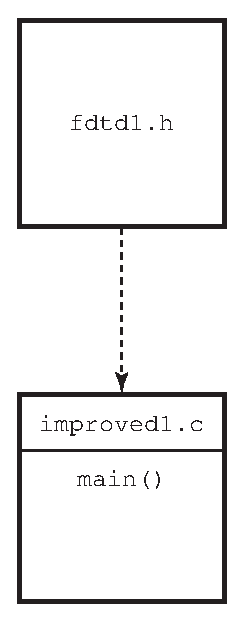
\epsfig{width=1.1in,file=Figures/Fdtd-improved-code/improved1-files.eps}
  \end{center} \caption{The files associated with the first improved
  version of the FDTD code.  The header file {\tt fdtd1.h} is included
  in the source file {\tt improved1.c} as indicated by the dashed
  line.  The source file {\tt improved1.c} contains the {\tt main()}
  function which performs all the executable statements associated with
  the simulation.}  \label{fig:improved1Files}
\end{figure}
The {\tt main()} function in file {\tt improved1.c} handles all the
calculations associated with the FDTD simulation.  Since there is only
a single source file, there is no obvious advantage to creating a
header file.  However, as we further modularize the code, the header
file will provide a convenient way to ensure that different source
files share common definitions of various things.  For example, many
source files may need to know about the details of a {\tt Grid}
structure.  These details can be written once in the header file and
then the header file can be included into different source files as
appropriate.  Examples of this will be provided in the following
sections.


\section{Modular Design and Initialization Functions\label{sec:modularDesign}}

Thus far all the programs have been written using a single source file
that contains a single function (the {\tt main()} function), or in the
case of the previous section, one source file and one header file.  As
the complexity of the FDTD simulation increases this approach becomes
increasingly unwieldy and error prone.  A better approach is to
modularize the program so that different functions perform specific
tasks---not everything is done within {\tt main()}.  For example, we
may want to use one function to update the magnetic field, another to
update the electric field, another to introduce energy into the grid,
and another to handle the termination of the grid.

Additionally, with C it is possible to put different functions in
different source files and compile the source files separately.  By
putting different functions in different source files, it is possible
to have different functions that are within one source file share
variables which are ``hidden'' from all functions that do not appear
in that file.  You can think of these variables as being private,
known only to the functions contained in the file.  As will be shown,
such sharing of variables can be useful when one wants to initialize
the behavior of a function that will be called multiple times (but the
initialization only needs to be done once).

To illustrate how functions within a file can share variables that are
otherwise hidden from other parts of a program, assume there is a
function that we want to call several times.  Further assume this
function performs a calculation based on some parameters but these
parameters only need to be set once---they will not vary from the
value to which they are initially set.  For this type of scenario, it
is often convenient to split the function into two functions: one
function handles the initialization of the parameters (the
``initialization function'') and the other function handles the
calculation based on those parameters (the ``calculation function'').
Now, the question is: How can the initialization function make the
parameters visible to the calculation function and how can the values
of these parameters persist between one invocation of the function and
the next?  The answer lies in global variables.

Generally the use of global variables is discouraged as they can make
programs hard to understand and difficult to debug.  However, global
variables can be quite useful when used properly.  To help minimize
the problems associated with global variables, we will further
modularizing the program so that the initialization function and
calculation function mentioned above are stored in a separate file
from the rest of the program.  In this way the global variables that
these functions share are not visible to any other function.

As a somewhat contrived example of this approach to setting
parameters, assume we want to write a program that will calculate the
values of a harmonic function where the user can specify the amplitude
and the phase, i.e., we want to calculate $f(x) = a\cos(x+\phi)$ where
$a$ is the amplitude and $\phi$ is the phase.  Note that we often just
write $f(x)$ for a function like this even though the function depends
on $a$ and $\phi$ as well as $x$.  We usually do {\em not} write
$f(x,a,\phi)$ because we think of $a$ and $\phi$ as fixed values (even
though they have to be specified at some point) while $x$ is the value
we are interested in varying.  Assume we want to write our program so
that there is a function {\tt harmonic1()} that is the equivalent of
$f(x) = a\cos(x+\phi)$.  {\tt harmonic1()} should take a single
argument that corresponds to the value of $x$.  We will use a separate
function, {\tt harmonicInit1()} that will set the amplitude and phase.

A file that contains a suitable the {\tt main()} function and the
associated statements to realize the parameter setting discussed above
is shown in Program \ref{pro:paramDemo1}.  The function prototypes for
{\tt harmonicInit1()} and {\tt harmonic1()} are given in lines
\ref{paramDemo1A} and \ref{paramDemo1B}, respectively.  Note, however,
that these functions do not appear in this file.  Between lines
\ref{paramDemo1C} and \ref{paramDemo1D} the user is prompted for the
amplitude and phase (and the phase is converted from degrees to
radians).  These values are passed as arguments to the {\tt
  harmonicInit1()} function.  As we will see a little later, this
function sets persistent global parameters to these values so that
they are visible to the function {\tt harmonic1()} whenever it is
called.  The for-loop that starts on line \ref{paramDemo1F} generates
the desired output values.  Here we set the variable {\tt x} to values
between $0$ and $2\pi$.  In line \ref{paramDemo1G} the value of {\tt x}
is printed together with the value of {\tt harmonic1(x)}.  Note that
the {\tt harmonic1()} function is not passed the amplitude or phase as
an argument.

\begin{program}
{\tt param-demo1.c}: File containing the {\tt main()} function and
appropriate header material that is used to demonstrate the setting of
persistent parameters in an auxilliary function.  Here {\tt
  harmonicInit1()} and {\tt harmonic1()} are serving this auxilliary
role.  The code associated with those functions is in a separate
file (see Program \ref{pro:harmonicDemo1}).
\label{pro:paramDemo1}
\codemiddle
\begin{lstlisting}
/* param-demo1.c:  Program that demonstrates the setting of
 * "persistent" parameters via the arguments of an initialization
 * function.  Here the parameters control the amplitude and phase of a
 * harmonic function f(x) = a cos(x + phi).  This program generates
 * num_points of the harmonic function with the "x" value of the
 * varying between zero and 2*pi.
 */

#include <stdio.h>
#include <math.h>  // To obtain M_PI, i.e., 3.14159...

void harmonicInit1(double amp, double phase);  /*@ \label{paramDemo1A} @*/
double harmonic1(double x);                    /*@ \label{paramDemo1B} @*/

int main() {
  double amp, phase, x;
  int mm, num_points = 100;

  printf("Enter the amplitude: ");       /*@ \label{paramDemo1C} @*/
  scanf(" %lf", &amp);
  printf("Enter the phase [in degrees]: ");
  scanf(" %lf", &phase);
  phase *= M_PI / 180.0;                 /*@ \label{paramDemo1D} @*/

  /* Set the amplitude and phase. */
  harmonicInit1(amp, phase);              /*@ \label{paramDemo1E} @*/

  for (mm = 0; mm < num_points; mm++) {   /*@ \label{paramDemo1F} @*/
    x = 2.0 * M_PI * mm / (float)(num_points - 1);
    printf("%f %f\n", x, harmonic1(x));  /*@ \label{paramDemo1G} @*/
  }

  return 0;
}
\end{lstlisting}
\end{program}

The file containing the functions {\tt harmonicInit1()} and {\tt
  harmonic1()} is shown in Program \ref{pro:harmonicDemo1}.  In line
\ref{paramDemo1A} two static double variables are declared: {\tt amp}
is the amplitude and {\tt phase} is the phase.  These variables are
visible to all the functions in this file but are not visible to any
other functions (despite the common name, these variables are distinct
from those with the same name in the {\tt main()} function).
Furthermore, the value of these variables will ``persist.''  They will
remain unchanged (unless we explicitly change them) and available for
our use through the duration of the running of the program.  (Note
that, it may perhaps be somewhat confusing, but the ``{\tt static}''
qualifier in line \ref{paramDemo1A} does not mean constant.  The value
of these variables can be changed.  Rather, it means these global
variables are local to this file.)

The {\tt harmonicInit1()} function starts on line \ref{harmonicDemo1B}.
It takes two arguments.  Here those arguments are labeled {\tt
  the\_amp} and {\tt the\_phase}.  We must distinguish these variable
names from the corresponding global variables.  We accomplish this by
putting the prefix {\tt the\_} on the corresponding global variable
name.  The global variables are set to the desired values in lines
\ref{harmonicDemo1C} and \ref{harmonicDemo1D}.  The {\tt harmonic1()}
function that begins on line \ref{harmonicDemo1E} then uses these
global values in the calculation of $a \cos(x+\phi)$.

\begin{program}
{\tt harmonic-demo1.c}: File containing the functions {\tt
  harmonicInit1()} and {\tt harmonic1()}.
\label{pro:harmonicDemo1}
\codemiddle
\begin{lstlisting}
/* 
 * harmonic-demo1.c: Functions to calculate a harmonic function of a
 * given amplitude and phase.  The desired amplitude and phase are
 * passed as arguments to harmonicInit1().  harmonicInit1() sets the
 * corresponding static global variables so that these values will be
 * available for the harmonic1() function to use whenever it is
 * called.
 */

#include <math.h> // for cos() function

/* Global static variables that are visible only to functions inside
   this file. */
static double amp, phase;     /*@ \label{harmonicDemo1A} @*/

// initialization function
void harmonicInit1(double the_amp, double the_phase) {  /*@ \label{harmonicDemo1B} @*/
  amp = the_amp;       /*@ \label{harmonicDemo1C} @*/
  phase = the_phase;   /*@ \label{harmonicDemo1D} @*/

  return;
}

// calculation function
double harmonic1(double x) {   /*@ \label{harmonicDemo1E} @*/
  return amp * cos(x + phase);
}
\end{lstlisting}
\end{program}

Now, let us change these programs in order to further separate the
{\tt main()} function from the harmonic function.  There is no reason
that the {\tt main()} function should have to prompt the user for the
amplitude or phase.  These values are simply passed along to the
harmonic initialization function and never actually used in {\tt
  main()}.  Thus, a better approach would be to let the harmonic
initialization function prompt the user for whatever input it needs.
The {\tt main()} function would merely call the initialization
function and leave all the details up to it.  So in the future, if one
wanted to change the harmonic function so the user could specify a
frequency as well as the amplitude and phase, that code could be added
to the harmonic functions but the {\tt main()} function would not have
to be changed in any way.

The new version of the {\tt main()} function is shown in Program
\ref{pro:paramDemo2}.  Note that there is now no mention of amplitude
or phase in {\tt main()}.  That information has all been relegated to
the harmonic functions themselves.

\begin{program}
  {\tt param-demo2.c}: Modified file containing the {\tt main()}
  function which demonstrates the use of an initialization function to
  set parameters.  In this version of the code the initilization
  function {\tt harmonicInit2()} takes no arguments.  The code for
  {\tt harmonicInit2()} and {\tt harmonic2()} is given in Program
  \ref{pro:harmonicDemo2}.
\label{pro:paramDemo2}
\codemiddle
\begin{lstlisting}
/* param-demo2.c: Program that demonstrates the setting of
 * "persistent" parameters via an initialization function.  Here the
 * initialization function handles all the details of obtaining the
 * parameters associated with the harmonic function.
 */

#include <stdio.h>
#include <math.h>  // To obtain M_PI, i.e., 3.14159...

void harmonicInit2();        /*@ \label{paramDemo2A} @*/
double harmonic2(double x);  /*@ \label{paramDemo2B} @*/

int main() {
  double x;
  int mm, num_points = 100;

  /* Initialize the harmonic function. */
  harmonicInit2();             /*@ \label{paramDemo2E} @*/

  for (mm = 0; mm < num_points; mm++) {   /*@ \label{paramDemo2F} @*/
    x = 2.0 * M_PI * mm / (float)(num_points - 1);
    printf("%f %f\n", x, harmonic2(x));  /*@ \label{paramDemo2G} @*/
  }

  return 0;
}
\end{lstlisting}
\end{program}

The file containing {\tt harmonicInit2()} and {\tt harmonic2()} is
shown in Program \ref{pro:harmonicDemo2}.  As before, the amplitude
and phase are global static variables that are declared in line
\ref{harmonicDemo2A}.  Note that {\tt harmonicInit2()} takes no
arguments.  Instead, this function prompts the user for the amplitude
and phase and sets the global variables appropriately.  Having done
this, these values are visible to the function {\tt harmonic2()}
(which is unchanged from the function {\tt harmonic1()} given
previously).

\begin{program}
{\tt harmonic-demo2.c}: File containing the functions {\tt
  harmonicInit2()} and {\tt harmonic2()}.
\label{pro:harmonicDemo2}
\codemiddle
\begin{lstlisting}
/* 
 * harmonic-demo2.c: Functions to calculate a harmonic function of a
 * given amplitude and phase.  harmonicInit2() prompts the user for
 * the amplitude and phase and sets the global variables so these
 * values will be available for the harmonic2() function to use
 * whenever it is called.
 */

#include <math.h> // for cos() function

/* Global static variables that are visible only to functions inside
   this file. */
static double amp, phase;     /*@ \label{harmonicDemo2A} @*/

// initialization function
void harmonicInit2() {  /*@ \label{harmonicDemo2B} @*/

  printf("Enter the amplitude: ");               /*@ \label{harmonicDemo2C} @*/
  scanf(" %lf", &amp);
  printf("Enter the phase [in degrees]: ");
  scanf(" %lf", &phase);
  phase *= M_PI / 180.0;                    /*@ \label{harmonicDemo2D} @*/

  return;
}

// calculation function
double harmonic2(double x) {   /*@ \label{harmonicDemo2E} @*/
  return amp * cos(x + phase);
}
\end{lstlisting}
\end{program}

In Sec.\ \ref{sec:compMultiFile} we will discuss the compilation of
multi-file programs such as these.


\section{Improvement Number Two}

Let us consider a further refinement to the simple bare-bones FDTD
simulation.  In this version of the code the updating of the electric
and magnetic fields will be handled by separate functions.  The grid
arrays will be initialized with a separate function and the source
function will be calculated using a separate function.  The
arrangement of the functions among the various files is depicted in
Fig.\ \ref{fig:improved2Files}.
\begin{figure}
  \begin{center}
  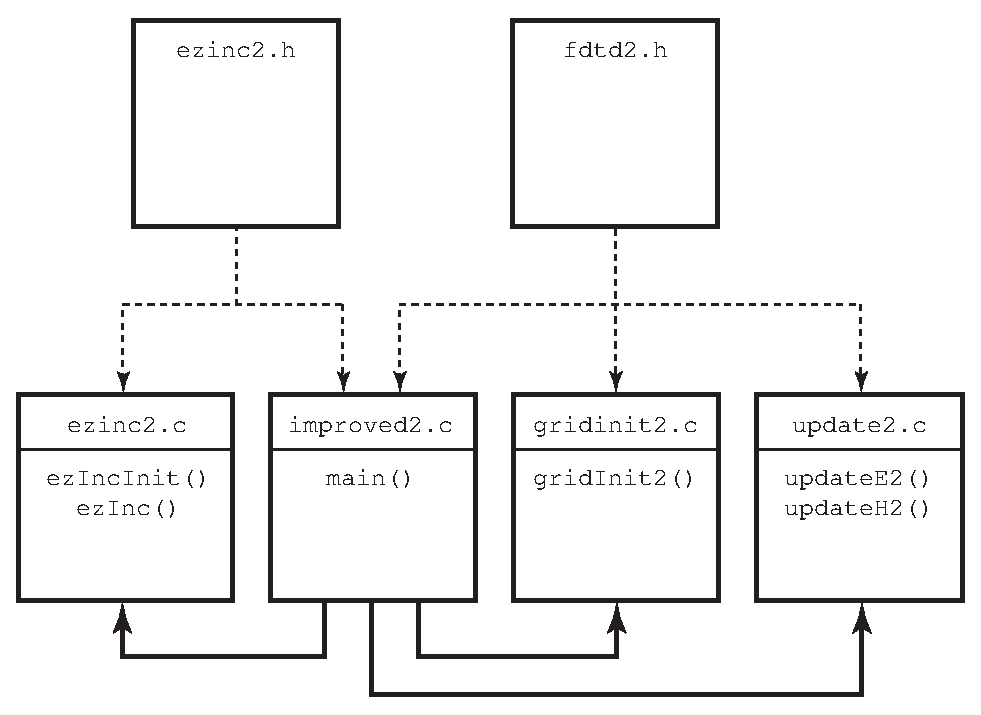
\epsfig{width=5.0in,file=Figures/Fdtd-improved-code/improved2-files.eps}
\end{center} \caption{The files associated with the second improved
  version of the FDTD code.  The header files {\tt fdtd2.h} and {\tt
    ezinc2.h} are included in the source files to which they are joined
  by a dashed line.  The file {\tt improved2.c} contains the {\tt
    main()} function but the initialization of the grid, the
  calculation of the source function, and the updating of the fields
  are no longer done in {\tt main()}.  Instead, other functions are
  called to accomplish these tasks.  The heavy black lines indicates
  which functions call which other functions.  In this case, {\tt
    main()} originates calls to all the other
  functions.}  \label{fig:improved2Files}
\end{figure}

Program \ref{pro:improved2} shows the contents of the file {\tt
  improved2.c}.  As indicated in Fig.\ \ref{fig:improved2Files}, {\tt
  main()} calls {\tt gridInit2()}.  This function initializes the {\tt
  Grid} structure {\tt g}.  The function {\tt gridInit2()} is
contained in the separate file {\tt gridinit2.c}.  The magnetic fields
are updated using the function {\tt updateH2()} while the electric
fields are updated using {\tt updateE2()}.  Both these functions are
contained in the file {\tt update2.c}.  The source function is
calculated using the function {\tt ezInc()} that is contained in the
file {\tt ezinc2.c}.

\begin{program} {\tt improved2.c}: Further code improvement of the
  bare-bones 1D FDTD simulation.  Here the initialization of the grid
  as well as the updating of the fields are handled by separate
  functions.  The argument for these functions is merely the {\tt
    Grid} pointer {\tt g}.  Additionally, the source function is
  initialized and calculated by separate
  functions. \label{pro:improved2} \codemiddle
\begin{lstlisting}
/* Version 2 of the improved bare-bones 1D FDTD simulation. */

#include "fdtd2.h"
#include "ezinc2.h"

int main()
{
  Grid *g;                             /*@ \label{improved2A} @*/

  ALLOC_1D(g, 1, Grid);       // allocate memory for Grid  /*@ \label{improved2B} @*/
  gridInit2(g);               // initialize the grid      /*@ \label{improved2C} @*/

  ezIncInit(g);               // initialize source function /*@ \label{improved2H} @*/

  /* do time stepping */
  for (Time = 0; Time < MaxTime; Time++) { /*@ \label{improved2D} @*/
    updateH2(g);              // update magnetic field  /*@ \label{improved2E} @*/
    updateE2(g);              // update electric field  /*@ \label{improved2F} @*/
    Ez(0) = ezInc(Time, 0.0); // apply source function  /*@ \label{improved2Z} @*/
    printf("%g\n", Ez(50));   // print output /*@ \label{improved2G} @*/
  } // end of time-stepping

  return 0;
}
\end{lstlisting}
\end{program}

Line \ref{improved2A} declares {\tt g} to be a pointer to a {\tt
  Grid}.  Since a {\tt Grid} structure has as elements the field
arrays, the time step, the duration of the simulations, and the
maximum number of time steps, none of these variables need to be
declared explicitly.  Note, however, that line \ref{improved2A} merely
creates a pointer but as yet this pointer does not point to anything
meaningful.  Line \ref{improved2B} uses {\tt ALLOC\_1D()} to allocated
memory for the {\tt Grid} and ensures {\tt g} points to that memory.
Assuming there were no errors in the allocation, this line is
effectively the equivalent of
\begin{code}
  g = calloc(1, sizeof(Grid));
\end{code}

As shown in lines \ref{improved2C}, \ref{improved2E}, and
\ref{improved2F}, {\tt gridInit2()}, {\tt updateH2()}, and {\tt
  updateE2()} each have a single argument: {\tt g} (a pointer to the
{\tt Grid}).  The parameters of the source function are initialized by
calling {\tt ezIncInit()} in line \ref{improved2H}.

The header file {\tt fdtd2.h} is shown in Program \ref{pro:fdtd2H}.
This file is largely the same as {\tt fdtd1.h}.  The only significant
difference is the function prototypes that are provided in lines
\ref{fdtd2HD}--\ref{fdtd2HF} for three of the functions called by {\tt
  main()} (note that the prototypes for the functions related to the
source are provided in {\tt ezinc2.h}).

\begin{program} {\tt fdtd2.h}: Header file to accompany the second
  version of the improved code showin in Program \ref{pro:improved2}.
  The differences between this file and {\tt fdtd1.h} are shown in
  bold. \label{pro:fdtd2H} \codemiddle
\begin{lstlisting}
/*b*/#ifndef _FDTD2_H
#define _FDTD2_H /*n*/

#include <stdio.h>
#include <stdlib.h>

struct Grid {
  double *ez;
  double *hy;
  int sizeX;
  int time, maxTime;
  double cdtds;
};

typedef struct Grid Grid;

/* memory allocation macro */
#define ALLOC_1D(PNTR, NUM, TYPE)                               \
    PNTR = (TYPE *)calloc(NUM, sizeof(TYPE));                   \
    if (!PNTR) {                                                \
      perror("ALLOC_1D");                                       \
      fprintf(stderr,                                           \
          "Allocation failed for " #PNTR ".  Terminating...\n");\
      exit(-1);                                                 \
    }

/* macros for accessing arrays and such */
#define Hy(MM)    g->hy[MM]
#define Ez(MM)    g->ez[MM]
#define SizeX     g->sizeX 
#define Time      g->time  
#define MaxTime   g->maxTime
#define Cdtds     g->cdtds

/*b*//* function prototypes */
void gridInit2(Grid *g);      /*@ \label{fdtd2HD} @*/
void updateH2(Grid *g);       /*@ \label{fdtd2HE} @*/
void updateE2(Grid *g);/*n*/  /*@ \label{fdtd2HF} @*/

#endif  /* matches #ifndef _FDTD2_H */
\end{lstlisting}
\end{program}

Program \ref{pro:update2} shows the contents of the file {\tt
  update2.c}.  The static global variable {\tt imp0} represents the
characteristic impedance of free space and is set to $377.0$ in line
\ref{update2A}.  This variable is never changed throughout the
program.  The magnetic field is updated with the function {\tt
  updateH2()} which is given between lines \ref{update2B} and
\ref{update2C}.  Note that the update equation uses {\tt Hy()} and
{\tt Ez()} to refer to the elements of the field arrays.  The macros
in {\tt fdtd2.h} translate these to the necessary syntax (which is
essentially {\tt g->hy[]} and {\tt g->ez[]}).  The electric field is
updated using {\tt updateE2()} which is given between lines
\ref{update2D} and \ref{update2F}.

\begin{program}
{\tt update2.c}: Source code for the functions {\tt updateH2()} and
{\tt updateE2()}. \label{pro:update2} 
\codemiddle
\begin{lstlisting}
/* Functions to update the electric and magnetic fields. */

#include "fdtd2.h"

/* characteristic impedance of free space */
static double imp0 = 377.0;  /*@ \label{update2A} @*/

/* update magnetic field */
void updateH2(Grid *g) {   /*@ \label{update2B} @*/
  int mm;

  for (mm = 0; mm < SizeX - 1; mm++)
    Hy(mm) = Hy(mm) + (Ez(mm + 1) - Ez(mm)) / imp0;

  return;
}                          /*@ \label{update2C} @*/

/* update electric field */
void updateE2(Grid *g) {   /*@ \label{update2D} @*/
  int mm;

  for (mm = 1; mm < SizeX - 1; mm++)
    Ez(mm) = Ez(mm) + (Hy(mm) - Hy(mm - 1)) * imp0;

  return;
}                          /*@ \label{update2F} @*/
\end{lstlisting}
\end{program}

Program \ref{pro:gridinit2} shows the source code for the function
{\tt gridInit2()}.  This function is used to set the value of various
elements of the {\tt Grid}.  (For this rather simple simulation, this
program is itself quite simple.)  Line \ref{gridinit2A} sets the size
of the Grid, {\tt SizeX}, to $200$.  Actually, after the preprocessor
has processed the code, this line will be
\begin{code}
  g->sizeX = 200;
\end{code}
Line \ref{gridinit2B} sets the duration of the simulation to $250$
time-steps.  Line \ref{gridinit2E} sets the Courant number to unity.
Lines \ref{gridinit2C} and \ref{gridinit2D} use the {\tt ALLOC\_1D()}
macro to allocate the necessary memory for the electric and magnetic
field arrays.

\begin{program}
{\tt gridinit2.c}: Source code for the function {\tt
gridInit2()}. \label{pro:gridinit2}
\codemiddle
\begin{lstlisting}
/* Function to initialize the Grid structure. */

#include "fdtd2.h"

void gridInit2(Grid *g) {
  SizeX = 200;                    // set the size of the grid /*@ \label{gridinit2A} @*/
  MaxTime = 250;                  // set duration of simulation /*@ \label{gridinit2B} @*/
  Cdtds = 1.0;                    // set Courant number /*@ \label{gridinit2E} @*/

  ALLOC_1D(g->ez, SizeX, double); // allocate memory for Ez /*@ \label{gridinit2C} @*/
  ALLOC_1D(g->hy, SizeX, double); // allocate memory for Hy /*@ \label{gridinit2D} @*/

  return;
}
\end{lstlisting}
\end{program}


Finally, Program \ref{pro:ezinc} shows the contents of the file {\tt
  ezinc2.c} which contains the code to implement the functions {\tt
  ezIncInit()} and {\tt ezInc()}.  The function {\tt ezinc()} is
Gaussian pulse whose width and delay are parameters that are set by
{\tt ezIncInit()}.  The implementation of this source function is
slightly different than in the original bare-bones code in that here
the user is prompted for the width and delay.  Additionally, the
source function {\tt ezInc()} takes two arguments, the time and the
location, so that this function can be used in a TFSF formulation.
When {\tt ezInc()} is called from {\tt main()}, the location is simply
hardwired to zero (ref.\ line \ref{improved2Z} of Program
\ref{pro:improved2}).

\begin{program} {\tt ezinc2.c}: File for the functions {\tt
    ezIncInit()} and {\tt ezInc()}.  {\tt ezInc()} is a traveling-wave
  implementation of a Gaussian pulse.  There are three private static
  global variables in this code.  These variables, representing the
  width and delay of the pulse as well as the Courant number, are
  determined and set by the initialization function {\tt ezIncInit()}.
  The Courant number is taken from the {\tt Grid} pointer that is
  passed as an argument while the user is prompted to provide the
  width and delay.
\label{pro:ezinc}
\codemiddle
\begin{lstlisting}
/* Functions to calculate the source function (i.e., the incident
 * field). */ 

#include "ezinc2.h"  /*@ \label{ezincY} @*/

/* global variables -- but private to this file */
static double delay, width = 0, cdtds;  /*@ \label{ezincX} @*/

/* prompt user for source-function width and delay. */
void ezIncInit(Grid *g){

  cdtds = Cdtds;  /*@ \label{ezincA} @*/
  printf("Enter delay: ");
  scanf(" %lf", &delay);
  printf("Enter width: ");
  scanf(" %lf", &width);

  return;
}

/* calculate source function at given time and location */
double ezInc(double time, double location) {
  if (width <= 0) {
    fprintf(stderr,
       "ezInc: must call ezIncInit before ezInc.\n"
       "       Width must be positive.\n");
    exit(-1);
  }
  return exp(-pow((time - delay - location / cdtds) / width, 2));
}
\end{lstlisting}
\end{program}

In Program \ref{pro:ezinc} the variable {\tt width} is used to
determine if initialization has been done.  {\tt width} is initialized
to zero when it is declared in line \ref{ezincX}.  If it is not
positive when {\tt ezInc()} is called, an error message is printed and
the program terminates.  In practice one should check that all the
parameters have been set to reasonable values, but here we only check
the width.

The private variable {\tt cdtds} declared in line \ref{ezincX} is
distinct from {\tt Cdtds} which the preprocessor expands to {\tt
  g->cdtds}.  That is to say the Courant number {\tt cdtds} that is an
element within the {\tt Grid} is different from the private variable
{\tt cdtds} in this file.  But, of course, we want these values to be
the same and line \ref{ezincA} assures this.

The header file to accompany {\tt ezinc2.c} is shown in Program {\tt
  ezinc2.h}.  As well as providing the necessary function prototypes,
this file ensures the inclusion of {\tt fdtd2.h} (which provides the
description a {\tt Grid} structure).

\begin{program}
{\tt ezinc2.h}: Header file that accompanies {\tt ezinc2.c} and is also
included in the file that specifies {\tt main()} (i.e., the file {\tt
  improved2.c}.
\label{pro:ezincH} 
\codemiddle
\begin{lstlisting}
/* Header file to accompany ezinc2.c. */

#ifndef _EZINC2_H   /*@ \label{ezincHA} @*/
#define _EZINC2_H   /*@ \label{ezincHB} @*/

#include <math.h>
#include <stdio.h>
#include <stdlib.h>
#include "fdtd2.h"   /*@ \label{ezincHC} @*/

void ezIncInit(Grid *g);
double ezInc(double time, double location);

#endif  /* matches #ifndef _EZINC2_H */          /*@ \label{ezincHD} @*/
\end{lstlisting}
\end{program}

\section{Compiling Modular Code \label{sec:compMultiFile}}

When a program is divided between multiple files it is typically not
necessary to recompile every file if there was a change in only some
of them.  Each source file can be compiled individually to an ``object
file'' or object code.  An object file, by itself, is not executable.
(To create executable code, all the object code must be linked
together.)  To create an object file with the GNU C compiler, one uses
the {\tt -c} flag.  Thus, for example, to obtain the object file for
{\tt ezinc2.c}, one would issue a command such as \index{gcc!object
  code}
\begin{code}
  gcc -Wall -O -c ezinc2.c
\end{code}
The flag {\tt -Wall} means to show all warnings, while {\tt -O} tells
the compiler to optimize the code (greater optimization can be
obtained by instead using {\tt -O2} or {\tt -O3}---the greater
optimization usually comes at the cost of slower compilation and larger
object and executable files).  When this command is issued the
compiler will create the object file {\tt ezinc2.o}.

The object files for all the components of the program can be created
separately by reissuing commands similar to the one shown above,
e.g., 
\begin{code}
  gcc -Wall -O -c ezinc2.c
  gcc -Wall -O -c improved2.c
  gcc -Wall -O -c update2.c
  gcc -Wall -O -c gridinit2.c
\end{code}
These commands would create the object files {\tt ezinc2.o}, {\tt
improved2.o}, {\tt update2.o}, and {\tt gridinit2.o}.  Alternatively,
one can create all the object files at once using a command such as
\begin{code}
  gcc -Wall -O -c ezinc2.c improved2.c update2.c gridinit2.c
\end{code}

\index{gcc!linking}
No matter how the object files are created, they need to be linked
together to obtain an executable.  The command to accomplish this is
\begin{code}
  gcc ezinc2.o improved2.o update2.o gridinit2.o -lm -o improved2
\end{code}
The flag {\tt -lm} tells the compiler to link to the math library
(which is necessary because of the math functions used in {\tt
ezinc2.c}).  The {\tt -o} flag allows one to specify the name of the
output/executable file, in this case {\tt improved2}.

For small programs there is not much advantage to incremental
compilation.  However, as the software increases in size and
complexity, there may be a significant savings in time realized by
recompiling only the code that has changed.  For example, assume a
change was made in the file {\tt gridinit2.c} but in no other.  Also
assume that the object code for each file has previously been created.
To obtain an executable that reflects this change one merely needs to
recompile this one file and then link the resulting object file to the
others, i.e.,
\begin{code}
  gcc -Wall -O -c gridinit2.c
  gcc ezinc2.o improved2.o update2.o gridinit2.o -lm -o improved2
\end{code}

\index{make}\index{makedepend} The details of incremental compilations
can actually be handled by utilities that detect the files that need
to be recompiled and react accordingly.  Those who are interested in
an example of such a utility may be interested in the {\tt make}
utility which is available on most Unix-based machines.  Another
helpful utility, which goes hand-in-hand with {\tt make} is {\tt
  makedepend} which sorts out the dependence of all the source files
on the header files.  {\tt make} is a rather old utility---going back
to the early days of Unix---and there are alternatives available such
as SCons available from \url{www.scons.org}.

\section{Improvement Number Three \label{sec:improveThree}}

Now let us modularize the program that contained the matched lossy
layer (Program \ref{pro:1Dmatched}).  As shown in Fig.\
\ref{fig:improvedFiles}, we will use separate functions for
initializing the grid, taking snapshots, applying the TFSF boundary,
updating the grid, and applying the ABC.  Additionally, the
calculation of the incident source function will be handled by a
separate function.  This source function will be called by the
function that implements the TFSF boundary, but no other.  Each box in
Fig.\ \ref{fig:improvedFiles} represents a separate file that contains
one or more functions.  The dashed lines indicate the inclusion of
header files and the heavy lines indicate function calls from one file
to another.

\begin{figure}
  \begin{center}
  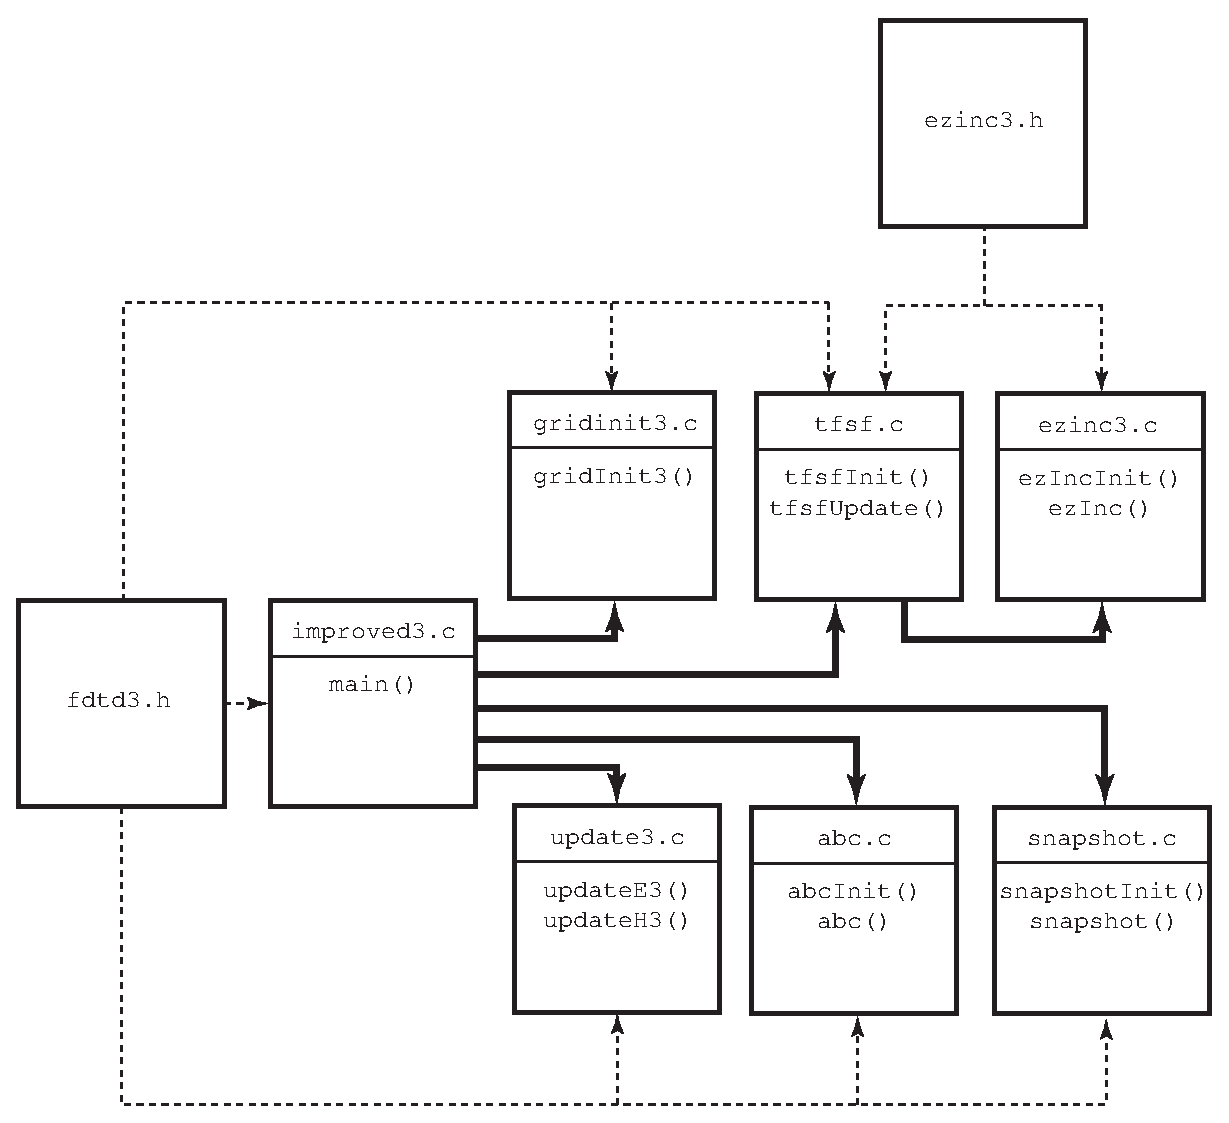
\epsfig{width=6.3in,file=Figures/Fdtd-improved-code/improved3-files.eps}
  \end{center} \caption{The files associated with the third
  improvement of the FDTD code.  The header file {\tt fdtd3.h} is
  explicitly included in the source files to which it is joined by a
  dashed line.  (Wherever {\tt ezinc3.h} appears it also ensures {\tt
  fdtd3.h} is included.)  The file {\tt improved3.c} contains the
  {\tt main()} function but the initialization of the grid, the
  application of the absorbing boundary condition, the calculation of
  the source function, the updating of the fields, and the taking of
  the snapshots is no longer done in {\tt main()}.  Instead, other
  functions are called to accomplish these tasks.}
  \label{fig:improvedFiles}
\end{figure}

The source code {\tt improved3.c} which contains the {\tt main()}
function is shown in Program \ref{pro:improved3}.  Note that nearly
all activities associated with the FDTD simulation are now done by
separate functions.  {\tt main()} merely serves to ensure that proper
initialization is done and then implements the time-stepping loop in
which the various functions are called.

\begin{program}
{\tt improved3.c}: Source code containing the {\tt main()} function.
Nearly all the FDTD related activities have been relegated to separate
functions which are called from {\tt main()}.  \label{pro:improved3}
\codemiddle
\begin{lstlisting}
/* FDTD simulation where main() is primarily used to call other
 * functions that perform the necessary operations. */

#include "fdtd3.h"

int main()
{
  Grid *g;

  ALLOC_1D(g, 1, Grid);  // allocate memory for Grid

  gridInit3(g);        // initialize the grid  /*@ \label{improved3A} @*/
  abcInit(g);          // initialize ABC       /*@ \label{improved3C} @*/
  tfsfInit(g);         // initialize TFSF boundary
  snapshotInit(g);     // initialize snapshots /*@ \label{improved3B} @*/

  /* do time stepping */
  for (Time = 0; Time < MaxTime; Time++) {
    updateH3(g);   // update magnetic field
    tfsfUpdate(g); // correct field on TFSF boundary
    abc(g);        // apply ABC
    updateE3(g);   // update electric field
    snapshot(g);   // take a snapshot (if appropriate)
  } // end of time-stepping

  return 0;
}
\end{lstlisting}
\end{program}

We have any number of options in terms of how functions should be
initialized or what arguments they should be passed.  Thus, one should
not consider this code to be optimum in any way.  Rather this code is
being used to illustrate implementation options.  

As in the previous program, {\tt main()} starts by defining a {\tt
  Grid} pointer and allocating space for the actual structure.  Then,
in lines \ref{improved3A}--\ref{improved3B}, four initialization
functions are called.  {\tt gridInit3()} initializes the {\tt Grid}
(this will be discussed in more detail shortly).  {\tt abcInit()}
handles any initialization associated with the ABC (as we will see, in
this particular case there is nothing for this initialization function
to do).  {\tt tfsfInit()} initializes the TFSF boundary while {\tt
  snapshotInit()} does the necessary snapshot initialization.
Following these initialization steps is the time-stepping loop where
the various functions are called that do the actual calculations.

The header {\tt fdtd3.h} is shown in Program \ref{pro:fdtd3h}.
Looking just at {\tt improved3.c} you would be unaware that the {\tt
  Grid} structure has changed.  However, four pointers have been added
that will contain the update-equation coefficients.  As can be seen in
lines \ref{fdtd3hA} and \ref{fdtd3hB} of Program \ref{pro:fdtd3h},
these pointers are named {\tt ceze}, {\tt cezh}, {\tt chyh}, and {\tt
  chye}.  Besides this and besides providing the function prototypes
for the new functions, this header file is largely the same as {\tt
  fdtd2.h}.
\begin{program}
{\tt fdtd3.h}: Header file to accompany {\tt improved3.c}.
Differences from {\tt fdtd2.h} are shown in bold.  \label{pro:fdtd3h}
\codemiddle
\begin{lstlisting}
/*b*/#ifndef _FDTD3_H
#define _FDTD3_H /*n*/

#include <stdio.h>
#include <stdlib.h>

struct Grid {
  double *ez, /*b*/*ceze, *cezh;/*n*/ /*@ \label{fdtd3hA} @*/
  double *hy, /*b*/*chyh, *chye;/*n*/ /*@ \label{fdtd3hB} @*/
  int sizeX;
  int time, maxTime;
  double cdtds;
};

typedef struct Grid Grid;

/* macros for accessing arrays and such */
#define Hy(MM)    g->hy[MM]
/*b*/#define Chyh(MM)  g->chyh[MM]
#define Chye(MM)  g->chye[MM]  /*n*/

#define Ez(MM)    g->ez[MM]
/*b*/#define Ceze(MM)  g->ceze[MM]
#define Cezh(MM)  g->cezh[MM]  /*n*/

#define SizeX     g->sizeX
#define Time      g->time
#define MaxTime   g->maxTime
#define Cdtds     g->cdtds

/* memory allocation macro */
#define ALLOC_1D(PNTR, NUM, TYPE)                               \
    PNTR = (TYPE *)calloc(NUM, sizeof(TYPE));                   \
    if (!PNTR) {                                                \
      perror("ALLOC_1D");                                       \
      fprintf(stderr,                                           \
          "Allocation failed for " #PNTR ".  Terminating...\n");\
      exit(-1);                                                 \
    }

/* Function prototypes */ /*b*/
void abcInit(Grid *g);
void abc(Grid *g);

void gridInit3(Grid *g);

void snapshotInit(Grid *g);
void snapshot(Grid *g);

void tfsfInit(Grid *g);
void tfsfUpdate(Grid *g);

void updateE3(Grid *g);
void updateH3(Grid *g); /*n*/

#endif  /* matches #ifndef _FDTD3_H */
\end{lstlisting}
\end{program}

The function {\tt gridInit3()} is contained in the file {\tt
  gridinit3.c} shown in Program \ref{pro:gridinit3}.  Keep in mind
that it does not matter what file names are---file names do not have
to match the contents of the file in any way, but, of course, it is
best to use names that are descriptive of the contents.

The preprocessor directives in lines
\ref{gridinit3A}--\ref{gridinit3B} are simply to provide convenient
names to the amount of loss, the starting location of the lossy layer,
and the relatively permittivity of the half space.  These parameters
are the same as they were in Program \ref{pro:1Dmatched}.

\begin{program} {\tt gridinit3.c}: The {\tt gridInit3()} function to
  initialize the {\tt Grid}.
\label{pro:gridinit3}
\codemiddle
\begin{lstlisting}
/* Function initialize Grid structure. */

#include "fdtd3.h"

#define LOSS 0.02       /*@ \label{gridinit3A} @*/
#define LOSS_LAYER 180  // node at which lossy layer starts
#define EPSR 9.0        /*@ \label{gridinit3B} @*/

void gridInit3(Grid *g) {
  double imp0 = 377.0;
  int mm;

  SizeX = 200;   // size of domain         /*@ \label{gridinit3C} @*/
  MaxTime = 450; // duration of simulation
  Cdtds = 1.0;   // Courant number         /*@ \label{gridinit3D} @*/

  ALLOC_1D(g->ez,   SizeX, double);  /*@ \label{gridinit3E} @*/
  ALLOC_1D(g->ceze, SizeX, double);
  ALLOC_1D(g->cezh, SizeX, double);
  ALLOC_1D(g->hy,   SizeX - 1, double);
  ALLOC_1D(g->chyh, SizeX - 1, double);
  ALLOC_1D(g->chye, SizeX - 1, double);  /*@ \label{gridinit3F} @*/
  
  /* set electric-field update coefficients */
  for (mm = 0; mm < SizeX; mm++)
    if (mm < 100) {
      Ceze(mm) = 1.0;
      Cezh(mm) = imp0;
    } else if (mm < LOSS_LAYER) {
      Ceze(mm) = 1.0;
      Cezh(mm) = imp0 / EPSR;
    } else {
      Ceze(mm) = (1.0 - LOSS) / (1.0 + LOSS);
      Cezh(mm) = imp0 / EPSR / (1.0 + LOSS);
    }

  /* set magnetic-field update coefficients */
  for (mm = 0; mm < SizeX - 1; mm++)
    if (mm < LOSS_LAYER) {
      Chyh(mm) = 1.0;
      Chye(mm) = 1.0 / imp0;
    } else {
      Chyh(mm) = (1.0 - LOSS) / (1.0 + LOSS);
      Chye(mm) = 1.0 / imp0 / (1.0 + LOSS);
    }

  return;
}
\end{lstlisting}
\end{program}

Lines \ref{gridinit3C}--\ref{gridinit3D} set the size of the {\tt
  Grid}, the duration of the simulation, and the Courant number.
Lines \ref{gridinit3E}--\ref{gridinit3F} allocate the necessary memory
for the various arrays.  The coefficient arrays are then set as they
were in Program \ref{pro:1Dmatched}.

The functions to update the electric and magnetic fields, i.e., {\tt
  updateE3()} and {\tt updateH3()} are contained in the file {\tt
  update3.c}.  The contents of this file are shown in Program
\ref{pro:update3}.  The functions are largely unchanged from those
that appeared in Program \ref{pro:update2}.  The only significant
differences are the appearance of the coefficient arrays in the update
equations that start on lines \ref{update3A} and \ref{update3B}.
\begin{program}
{\tt update3.c}: Functions to update the electric and magnetic fields.
\label{pro:update3}
\codemiddle
\begin{lstlisting}
/* Functions to update the electric and magnetic fields. */

#include "fdtd3.h"

/* update magnetic field */
void updateH3(Grid *g) {
  int mm;

  for (mm = 0; mm < SizeX - 1; mm++)
    Hy(mm) = Chyh(mm) * Hy(mm) +          /*@ \label{update3A} @*/
             Chye(mm) * (Ez(mm + 1) - Ez(mm));

  return;
}

/* update electric field */
void updateE3(Grid *g) {
  int mm;

  for (mm = 1; mm < SizeX - 1; mm++)
    Ez(mm) = Ceze(mm) * Ez(mm) +      /*@ \label{update3B} @*/
             Cezh(mm) * (Hy(mm) - Hy(mm - 1));

  return;
}
\end{lstlisting}
\end{program}

The function to apply the absorbing boundary conditions is rather
trivial and is shown in Program \ref{pro:abcTrivial}.  Also shown in
Program \ref{pro:abcTrivial} is the initiliztaion function {\tt
  abcInit()}.  In this particular case the ABC is so simple that there
is no initializataion that needs to be done and hence this function
simply returns.  In Chap.\ \ref{chap:abc} we will begin to consider more
sophisticated ABC's that do indeed require some initialization.  Thus,
this call the initialization function is done in anticipation of that.
As was the case in Program \ref{pro:1Dmatched}, the ABC is only
applied to the left side of the grid.  The right side of the grid is
terminated with a lossy layer.

\begin{program}
{\tt abc.c}: Absorbing boundary condition used by {\tt improved3.c}.
For this particular simple ABC there is nothing for the initialization
function to do and hence it simply returns.
\label{pro:abcTrivial}
\codemiddle
\begin{lstlisting}
/* Functions to terminate left side of grid. */

#include "fdtd3.h"

// Initialize the ABC -- in this case, there is nothing to do.
void abcInit(Grid *g) {

  return;
}

// Apply the ABC -- in this case, only to the left side of grid.
void abc(Grid *g) {

  /* simple ABC for left side of grid */
  Ez(0) = Ez(1);

  return;
}
\end{lstlisting}
\end{program}

The code associated with the TFSF boundary is shown in Program
\ref{pro:tfsfTrivial}.  Line \ref{tfsfTrivA} declares a static global
variable {\tt tfsfBoundary} which specifies the location of the TFSF
boundary.  This variable is initialized to zero with the understanding
that when the code is initialized it will be set to some meaningful
(positive) value.

\begin{program}
{\tt tfsf.c}: Code to implement the TFSF boundary.
\label{pro:tfsfTrivial}
\codemiddle
\begin{lstlisting}
/* Function to implement a 1D FDTD boundary. */

#include <math.h>
#include "fdtd3.h"
#include "ezinc3.h"

static int tfsfBoundary = 0;  /*@ \label{tfsfTrivA} @*/

void tfsfInit(Grid *g) {    /*@ \label{tfsfTrivB} @*/

  printf("Enter location of TFSF boundary: ");
  scanf(" %d", &tfsfBoundary);

  ezIncInit(g); // initialize source function /*@ \label{tfsfTrivD} @*/

  return;
}

void tfsfUpdate(Grid *g) {   /*@ \label{tfsfTrivE} @*/
  /* check if tfsfInit() has been called */
  if (tfsfBoundary <= 0) {
    fprintf(stderr,
      "tfsfUpdate: tfsfInit must be called before tfsfUpdate.\n"
      "            Boundary location must be set to positive value.\n");
    exit(-1);
  }

  /* correct Hy adjacent to TFSF boundary */
  Hy(tfsfBoundary) -= ezInc(Time, 0.0) * Chye(tfsfBoundary);
    
  /* correct Ez adjacent to TFSF boundary */
  Ez(tfsfBoundary + 1) += ezInc(Time + 0.5, -0.5);
  
  return;
}
\end{lstlisting}
\end{program}

The initialization function {\tt tfsfInit()} begins on line
\ref{tfsfTrivB}.  The user is prompted to enter the location of the
TFSF boundary.  Then the initialization function for the source {\tt
  ezIncInit()} is called to set the parameters that control the shape
of the pulse.  

The code to calculate the source function, i.e., the functions {\tt
  ezIncInit()} and {\tt ezInc()} is identical to that shown in Program
\ref{pro:ezinc}.  However, there would be one slight change to the
file: instead of including {\tt ezinc2.h}, line \ref{ezincY} of
Program \ref{pro:ezinc} would be changed to include {\tt ezinc3.h}.
We assume this modified program is in the file {\tt ezinc3.c} which is
not shown.  The header file {\tt ezinc3.h} would be nearly identical
to the code shown in Program \ref{pro:ezincH} except the ``$2$'' in
lines \ref{ezincHA}, \ref{ezincHB}, and \ref{ezincHC}, would be
changed to ``$3$'' (thus ensuring the proper inclusion of the header
file {\tt fdtd3.h} instead of {\tt fdtd2.h}).  Again, since this is
such a minor change, the contents of {\tt ezinc3.h} are not shown.

The function {\tt tfsfUpdate()} which begins on line \ref{tfsfTrivE}
is called once every time-step.  This function applies the necessary
correction to the nodes adjacent to the TFSF boundary.  Because of the
implicit timing within this file, this function needs to be called
after the magnetic-field update, but before the electric-field update.
The function first checks that the boundary location is positive.  If
it is not, an error message is printed and the program terminates,
otherwise the fields adjacent to the boundary are corrected.

Finally, the code associated with taking snapshots of the field is
shown in Program \ref{pro:snapTrivial}.  {\tt snapshotInit()} allows
the user to specify the time at which snapshots should start, the
temporal stride between snapshots, the node at which a snapshot should
start, the node at which it should end, the spatial stride between
nodes, and the base name of the output files.  Assuming the user
entered a base name of {\tt sim}, then, as before, the output files
would be named {\tt sim.0}, {\tt sim.1}, {\tt sim.2}, and so on.  If
the user said the {\tt startTime} is $105$ and the {\tt
temporalStride} is $10$, then snapshots would be taken at time-steps
$105$, $115$, $125$, and so on.  Similarly, if the user specified that
the {\tt startNode} and {\tt endNode} are $0$ and $180$, respectively,
and the {\tt spatialStride} is $1$, then the value of every node
between $0$ and $180$, inclusive, would be recorded to the snapshot
file.  If the {\tt spatialStride} were $2$, every other node would be
recorded.  If it were $3$, every third node would be recorded.
(Because of this, the {\tt endNode} only corresponds to the actual
last node in the snapshot file if its offset from the {\tt startNode}
is an even multiple of the spatial stride.)

\begin{program}
{\tt snapshot.c}: Code for taking snapshots of the electric field.
\label{pro:snapTrivial}
\codemiddle
\begin{lstlisting}
/* Function to take a snapshot of a 1D grid. */

#include "fdtd3.h"

static int temporalStride = 0, spatialStride, startTime,
  startNode, endNode, frame = 0;
static char basename[80];

void snapshotInit(Grid *g) { /*@ \label{snapTrivA} @*/
  
  printf("For the snapshots:\n");
  printf("  Duration of simulation is %d steps.\n", MaxTime);
  printf("  Enter start time and temporal stride: ");
  scanf(" %d %d", &startTime, &temporalStride);
  printf("  Grid has %d total nodes (ranging from 0 to %d).\n",
	 SizeX, SizeX-1);
  printf("  Enter first node, last node, and spatial stride: ");
  scanf(" %d %d %d", &startNode, &endNode, &spatialStride);
  printf("  Enter the base name: ");
  scanf(" %s", basename);

  return;
}

void snapshot(Grid *g) { /*@ \label{snapTrivB} @*/
  int mm;
  char filename[100];
  FILE *snapshot;

  /* ensure temporal stride set to a reasonable value */
  if (temporalStride <= 0) {
    fprintf(stderr,
      "snapshot: snapshotInit must be called before snapshot.\n"
      "          Temporal stride must be set to positive value.\n");
    exit(-1);
  }

  /* get snapshot if temporal conditions met */
  if (Time >= startTime && 
      (Time - startTime) % temporalStride == 0) {
    sprintf(filename, "%s.%d", basename, frame++);
    snapshot = fopen(filename, "w");
    for (mm = startNode; mm <= endNode; mm += spatialStride)
      fprintf(snapshot, "%g\n", Ez(mm));
    fclose(snapshot);
  }

  return;
}
\end{lstlisting}
\end{program}

As shown in line \ref{snapTrivA}, {\tt snapshotInit()} takes a single
argument, a pointer to a {\tt Grid} structure.  This function prompts
the user to set the appropriate snapshot control values.  The snapshot
files themselves are created by the function {\tt snapshot()} which
starts on line \ref{snapTrivB}.  This function starts by checking that
the temporal stride has been set to a reasonable value.  If not, an
error message is printed and the program terminates.  The program then
checks if time is greater than or equal to {\tt startTime} and the
difference between the current time and the {\tt startTime} is a
multiple of {\tt temporalStride}.  If not, the function returns.  If
those conditions are met, then, as we have seen before, a snapshot
file is written and the frame counter is advanced.  However, now there
is some control over which nodes are actually written.  Note that the
function {\tt snapshot()} is called every time-step.  We could easily
have checked in the {\tt main()} function if the time-step was such
that a snapshot should be generated and only then called {\tt
  snapshot()}.  Reasons for adopting either approach could be made but
be aware that the overhead for calling a function is typically small.
Thus, the savings realized by calling {\tt snapshot()} less often (but
still ultimately generating the same number of snapshots) is likely to
be trivial.  The approach used here keeps all the snapshot-related
data in the snapshot code itself.

After compiling all this code (and linking it), the executable will
produce the same results as were obtained from Program
\ref{pro:1Dmatched} (assuming, of course, the user enters the same
parameters as were used in Program \ref{pro:1Dmatched}).  With the new
version of the code there are several improvements we could
potentially use to our advantage.  Assume, for instance, we wanted to
do simulations of two different scenarios.  We could create two {\tt
  Grid} structures, one for scenario.  Each grid would have its own
{\tt gridInit()} function, but other than that all the code could be
used by either grid.  The update functions could be applied, without
any modification, to any grid.  The snapshot function could be applied
to any grid, and so on.


